\documentclass[]{article}
\usepackage{lmodern}
\usepackage{amssymb,amsmath}
\usepackage{ifxetex,ifluatex}
\usepackage{fixltx2e} % provides \textsubscript
\ifnum 0\ifxetex 1\fi\ifluatex 1\fi=0 % if pdftex
  \usepackage[T1]{fontenc}
  \usepackage[utf8]{inputenc}
\else % if luatex or xelatex
  \ifxetex
    \usepackage{mathspec}
  \else
    \usepackage{fontspec}
  \fi
  \defaultfontfeatures{Ligatures=TeX,Scale=MatchLowercase}
  \newcommand{\euro}{€}
\fi
% use upquote if available, for straight quotes in verbatim environments
\IfFileExists{upquote.sty}{\usepackage{upquote}}{}
% use microtype if available
\IfFileExists{microtype.sty}{%
\usepackage{microtype}
\UseMicrotypeSet[protrusion]{basicmath} % disable protrusion for tt fonts
}{}
\usepackage[margin=1in]{geometry}
\usepackage{hyperref}
\PassOptionsToPackage{usenames,dvipsnames}{color} % color is loaded by hyperref
\hypersetup{unicode=true,
            pdftitle={About Writing Dynamic Documents with R},
            pdfauthor={Author Name1; 1Department of Geography, University of Zurich, Winterthurerstrasse 190, Zurich; name@geo.uzh.ch},
            pdfborder={0 0 0},
            breaklinks=true}
\urlstyle{same}  % don't use monospace font for urls
\usepackage{longtable,booktabs}
\usepackage{graphicx,grffile}
\makeatletter
\def\maxwidth{\ifdim\Gin@nat@width>\linewidth\linewidth\else\Gin@nat@width\fi}
\def\maxheight{\ifdim\Gin@nat@height>\textheight\textheight\else\Gin@nat@height\fi}
\makeatother
% Scale images if necessary, so that they will not overflow the page
% margins by default, and it is still possible to overwrite the defaults
% using explicit options in \includegraphics[width, height, ...]{}
\setkeys{Gin}{width=\maxwidth,height=\maxheight,keepaspectratio}
\setlength{\parindent}{0pt}
\setlength{\parskip}{6pt plus 2pt minus 1pt}
\setlength{\emergencystretch}{3em}  % prevent overfull lines
\providecommand{\tightlist}{%
  \setlength{\itemsep}{0pt}\setlength{\parskip}{0pt}}
\setcounter{secnumdepth}{0}

%%% Use protect on footnotes to avoid problems with footnotes in titles
\let\rmarkdownfootnote\footnote%
\def\footnote{\protect\rmarkdownfootnote}

%%% Change title format to be more compact
\usepackage{titling}

% Create subtitle command for use in maketitle
\newcommand{\subtitle}[1]{
  \posttitle{
    \begin{center}\large#1\end{center}
    }
}

\setlength{\droptitle}{-2em}
  \title{About Writing Dynamic Documents with R}
  \pretitle{\vspace{\droptitle}\centering\huge}
  \posttitle{\par}
  \author{Author Name\textsuperscript{1} \\ \textsuperscript{1}Department of Geography, University of Zurich,
Winterthurerstrasse 190, Zurich \\ \href{mailto:name@geo.uzh.ch}{\nolinkurl{name@geo.uzh.ch}}}
  \preauthor{\centering\large\emph}
  \postauthor{\par}
  \date{}
  \predate{}\postdate{}



% Redefines (sub)paragraphs to behave more like sections
\ifx\paragraph\undefined\else
\let\oldparagraph\paragraph
\renewcommand{\paragraph}[1]{\oldparagraph{#1}\mbox{}}
\fi
\ifx\subparagraph\undefined\else
\let\oldsubparagraph\subparagraph
\renewcommand{\subparagraph}[1]{\oldsubparagraph{#1}\mbox{}}
\fi

\begin{document}
\maketitle
\begin{abstract}
This is the abstract of the template document used to show how to write
publications in R with R Markdown and the help of some packages. Based
on a concrete use case, this document exemplifies some of the caveats
that may occur when writing such a document and publishing it online on
a Git repository. It also presents typical use cases in Markdown usage
and presents some tricks.
\end{abstract}

\subsection{Introduction}\label{introduction}

This example publication serves as a motivation on how to create
reproducible documents in R and aims to promote reproducible research in
general.

\subsection{State of the Art}\label{state-of-the-art}

Various authors in qualitative and quantitive research argue that as
many parts of the research workflow as possible should be reproducible.
Brunsdon (2015) state ``Reproducible quantitative research is research
that has been documented sufficiently rigorously that a third party can
replicate any quantitative results that arise''.

To further motivate you, read (Buckheit and Donoho 1995, Healy 2011,
2016, Nüst \emph{et al.} 2011, LeVeque \emph{et al.} 2012, Pebesma
\emph{et al.} 2012, Vandewalle 2012, Baker 2016, Editorial 2016) or the
short and to the point editorial from Editorial (2016).

\subsection{Case Study: Parc Adula}\label{case-study-parc-adula}

This case study presents a small subset of data from a current study
conducted at the Department of Geography at the University of Zurich.
The study investigates social negotiations revolving around a national
park project in Switzerland -- \emph{Parc Adula} -- and aims for a
better understanding of how people reason in a public environmental
debate.

\subsubsection{Exploratory topic
analysis}\label{exploratory-topic-analysis}

For this case study, 16 interviews were carried out. Each of these
semi-structured interviews was analyzed resorting to Mayring's
qualitative content analysis (Mayring and Fenzl (2014)) -- resulting in
a code system, which was derived through mainly inductive category
development. The following plots display sample output from the MXAQDA
software for qualitative data analysis.

Overview of the interviews and representatives:

\begin{itemize}
\tightlist
\item
  \emph{Cantonal Goverment} (n: 4): Representatives from four different
  departments
\item
  \emph{Environmental Organisation} (n: 1): Representative from a
  specific interest group with advisory function.
\item
  \emph{Federal Goverment} (n: 2): Must ensure the park follows the laws
  and decrees
\item
  \emph{Local} (n: 5): Local representatives of the park region
\item
  \emph{Parc Team} (n: 2): Team members involved in the park planning
  process
\item
  \emph{Tourism} (n: 2): Local tourism representatives
\end{itemize}

The following plot presents the frequency of occurence of a select list
of topics that occured in the interviews. While there seems to be more
focus on the \emph{Pro Argument} against the \emph{Contra Argument}
during the interviews, topics on \emph{Tourismus} seem to have far more
weight than those on \emph{Biodiversität}.

\begin{longtable}[c]{@{}lr@{}}
\caption{Topic mentions.}\tabularnewline
\toprule
Code & Mention\tabularnewline
\midrule
\endfirsthead
\toprule
Code & Mention\tabularnewline
\midrule
\endhead
Biodiversitaet & 5\tabularnewline
Contra Argument & 39\tabularnewline
Pro Argument & 68\tabularnewline
Tourismus allgemein & 48\tabularnewline
\bottomrule
\end{longtable}

The next figure presents the frequency matrix of the topic occurences
across the different interviews. It provides an overview of where topics
are mentioned and by whom.

\begin{figure}[htbp]
\centering
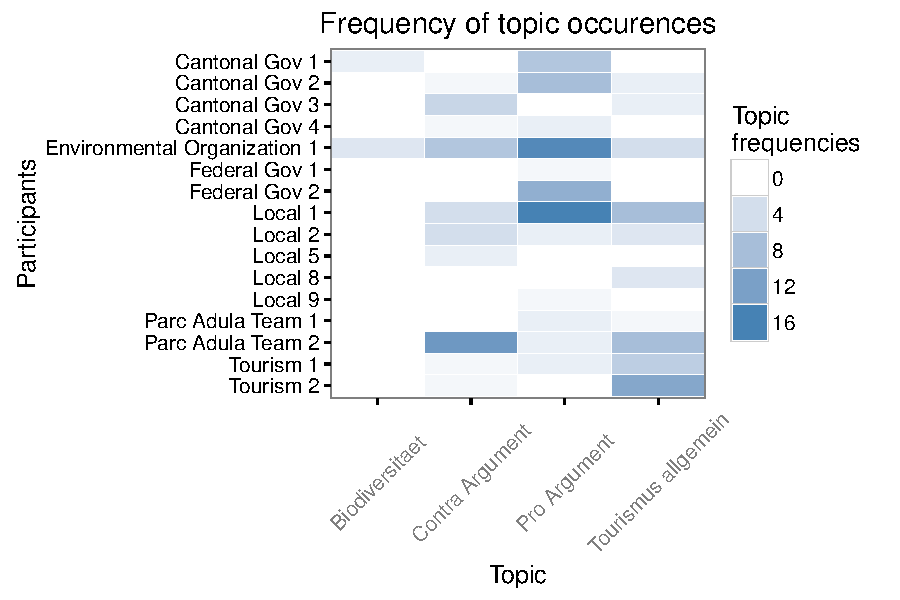
\includegraphics{publication_files/figure-latex/plotfreq-1.pdf}
\caption{Frequency matrix of a selected list of topics across the
various representants}
\end{figure}

\textbf{Notes on reproducibility:} Depending on the data to analyze,
privacy may play a role. While for the analysis itself the data is being
anonymised, storing the raw or preprocessed data on a public repository
may pose privacy issues or even constitute a violation of contract.

\subsubsection{Google query timeline}\label{google-query-timeline}

Overview of the Google trend evolution of the search query: \emph{Parc
Adula}
(\href{https://www.google.com/trends/explore?date=all\&q=parc\%20adula}{url},
provides a CSV file). The timeline shows overall a small amount of
queries for this word combination, with a spike on 2015-11-01. This was
retrieved on August 11, 2016.

\textbf{Notes on reproducibility:} Web APIs are subject to license
restrictions, can get altered by the service provider, or can simply
cease to exist, so consider them carefully before using them in a
scientific project. Consider instead using software which you can store
locally and can better control the parameters and settings. If
collecting data from an API, ensure to note down as much as possible
about the data collection: the date range, all the query parameters,
including the service limits at the time, any interruptions in service,
and so on. It's also wise to back up the data thus obtained, if at all
possible!

\begin{figure}[htbp]
\centering
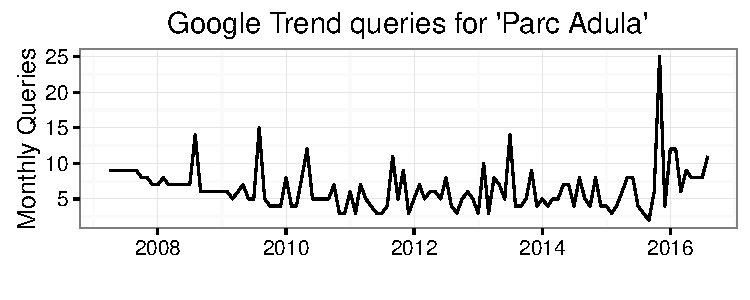
\includegraphics{publication_files/figure-latex/googleTrend-1.pdf}
\caption{Timeline of queries for Parc Adula set in the Google search
engine}
\end{figure}

\subsubsection{Case study area}\label{case-study-area}

The proposed Parc Adula national park candidate is situated in
Switzerland in the border region of the cantons Ticino and Grisons
(Graubünden). The map below presents the current outer perimiter of the
planned national park.

\textbf{Notes on reproducibility:} Due to license restrictions of the
open geodata, it is not possible to store the data on a public Git
repository. The included script \texttt{R/loadMapData.r} downloads the
data directly from the link provided in the geodata catalog infobox of
\url{http://maps.geo.admin.ch}

\begin{figure}
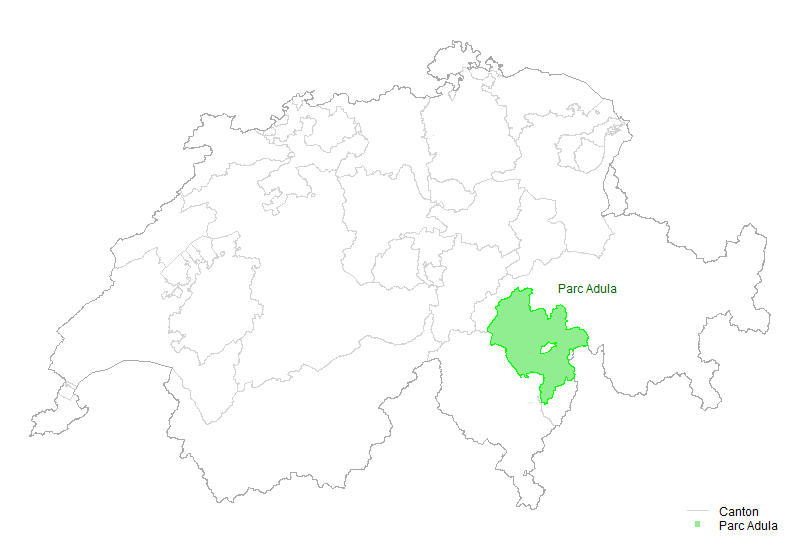
\includegraphics[width=0.6\linewidth]{figures/map} \caption{Planned perimeter of Parc Adula, Switzerland, Data source: Swisstopo}\label{fig:map}
\end{figure}

\subsection{Concluding discussion}\label{concluding-discussion}

This template is based on data from an ongoing research project and
presents some typical examples of material that could be used in a
publication written in RMarkdown. It shows how to include data and
analyses, features plots, tables, literature, and various markdown
elements. The generated files in \emph{PDF}, \emph{Word} or \emph{HTML}
often still need some fine-tuning afterwards (particularly in Latex). It
is nevertheless a great way of documenting the research process,
generating initial drafts, and sharing workflows with collaborators or a
wider audience.

\section{Acknowledgements}\label{acknowledgements}

The Reproducible Research workshop was supported by the InnoPool fund of
the Department of Geography, University of Zurich.

\section*{References}\label{references}
\addcontentsline{toc}{section}{References}

\hypertarget{refs}{}
\hypertarget{ref-Baker2016}{}
Baker, M., 2016. 1,500 scientists lift the lid on reproducibility.
\emph{Nature}, 533 (7604), 452--454.

\hypertarget{ref-Brunsdon2015}{}
Brunsdon, C., 2015. Quantitative methods I: Reproducible research and
quantitative geography. \emph{Progress in Human Geography}.

\hypertarget{ref-Buckheit1995}{}
Buckheit, J. and Donoho, D., 1995. WaveLab and Reproducible Research.
\emph{Wavelets and Statistics}, 103, 55--81.

\hypertarget{ref-Nature2016}{}
Editorial, 2016. Reality check on reproducibility. \emph{Nature}, 533
(7604), 437--437.

\hypertarget{ref-Healy2011}{}
Healy, K., 2011. Choosing Your Workflow Applications. \emph{The
Political Methodologist}, 18 (2), 9--18.

\hypertarget{ref-Healy2016}{}
Healy, K., 2016. \emph{The Plain Person's Guide to Plain Text Social
Science}. Healy2016.

\hypertarget{ref-Leveque2012}{}
LeVeque, R.J., Mitchell, I.M., and Stodden, V., 2012. Reproducible
research for scientific computing: Tools and strategies for changing the
culture. \emph{Computing in Science \& Engineering}, 14 (4), 13--17.

\hypertarget{ref-Mayring2010}{}
Mayring, P. and Fenzl, T., 2014. Qualitative inhaltsanalyse, 601--613.

\hypertarget{ref-Nuest2011}{}
Nüst, D., Stasch, C., and Pebesma, E., 2011. Connecting R to the sensor
Web. \emph{In}: \emph{Lecture notes in geoinformation and cartography}.
227--246.

\hypertarget{ref-Pebesma2012}{}
Pebesma, E., Nüst, D., and Bivand, R., 2012. The R software environment
in reproducible geoscientific research. \emph{Eos, Transactions American
Geophysical Union}, 93 (16), 163--163.

\hypertarget{ref-Vandewalle2012}{}
Vandewalle, P., 2012. Code Sharing Is Associated with Research Impact in
Image Processing. \emph{Computing in Science \& Engineering}, 14 (4),
42--47.

\end{document}
